\documentclass{beamer}

\usepackage{hyperref} 
\usepackage{graphicx}

\begin{document}

\begin{frame}{Zes personen op een rijtje...}

\only<1>{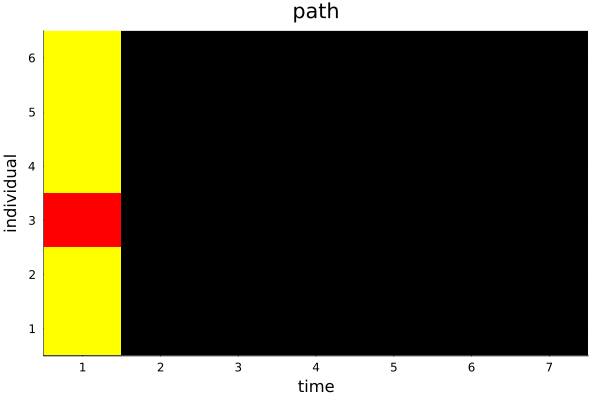
\includegraphics[scale=0.5]{smallexample1.png} }
\only<2>{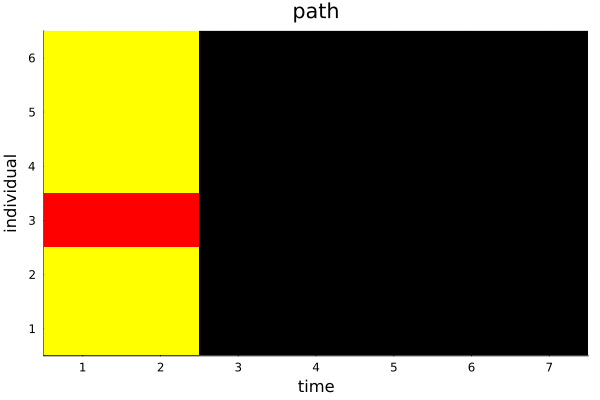
\includegraphics[scale=0.5]{smallexample2.png} }	
\only<3>{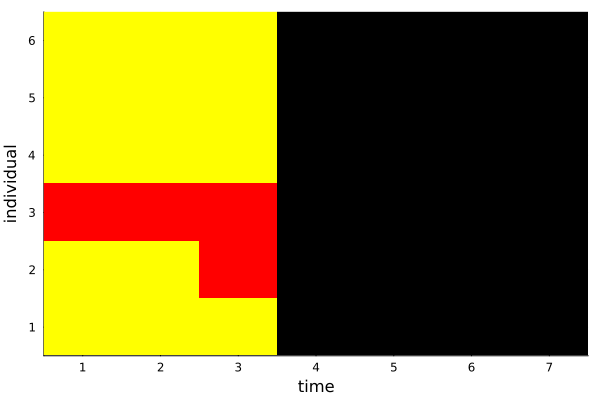
\includegraphics[scale=0.5]{smallexample3.png} }	
\only<4>{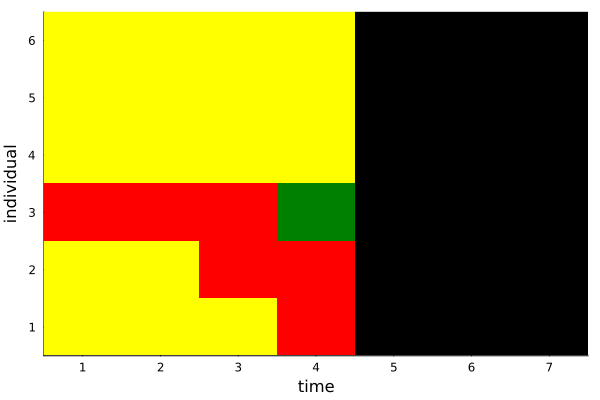
\includegraphics[scale=0.5]{smallexample4.png} }	
\only<5>{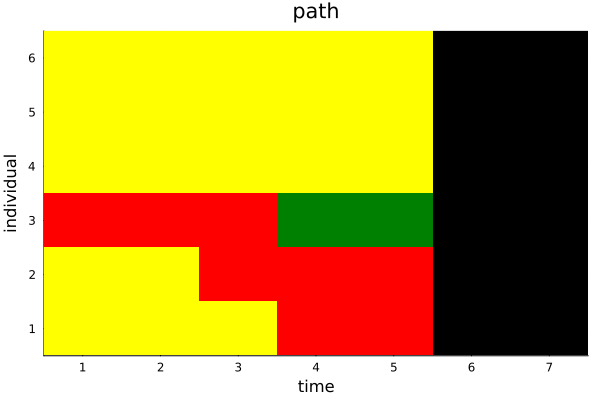
\includegraphics[scale=0.5]{smallexample5.png} }	
\only<6>{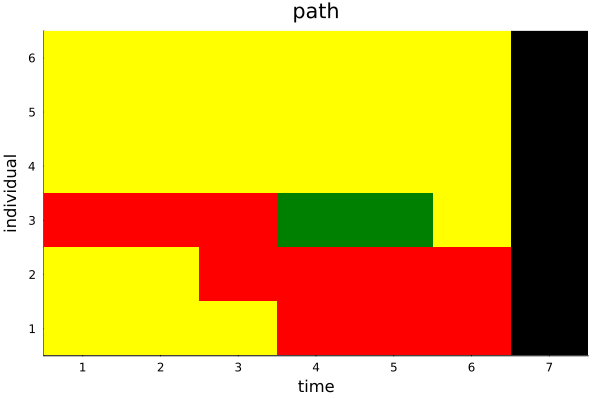
\includegraphics[scale=0.5]{smallexample6.png} }	
\only<7>{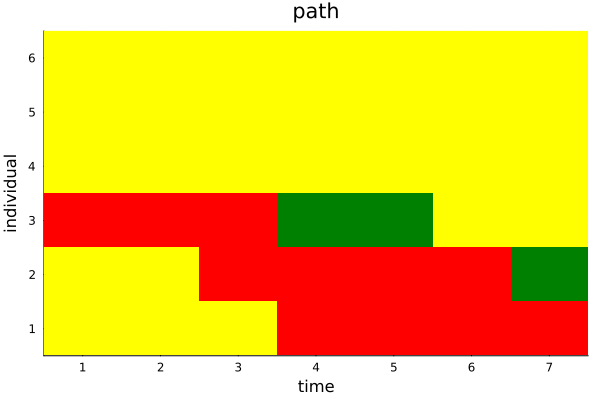
\includegraphics[scale=0.5]{smallexample7.png} }	
\end{frame}



   
\begin{frame}{Stochastische simulatie: alles bij elkaar...}

 \href{run:smallexample.mp4}{Click here to play the video}
	
\end{frame}


\begin{frame}{Een wat groter voorbeeld}
\begin{itemize}
	\item 50 personen
	\item 100 tijdstappen
\end{itemize}	



 \href{run:large_example.mp4}{Click here to play the video}
\end{frame}



\begin{frame}{Andere realisaties}



\only<1>{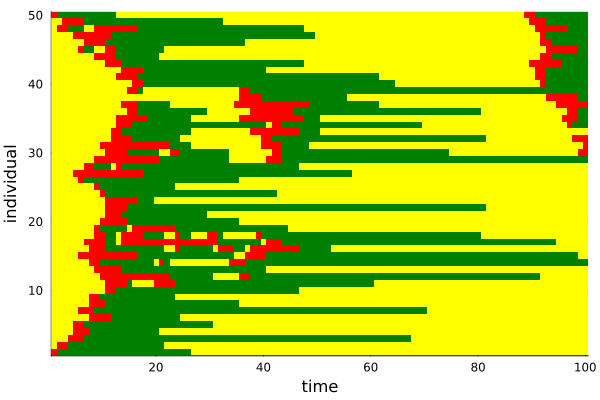
\includegraphics[scale=0.5]{large_example1.png} }
\only<2>{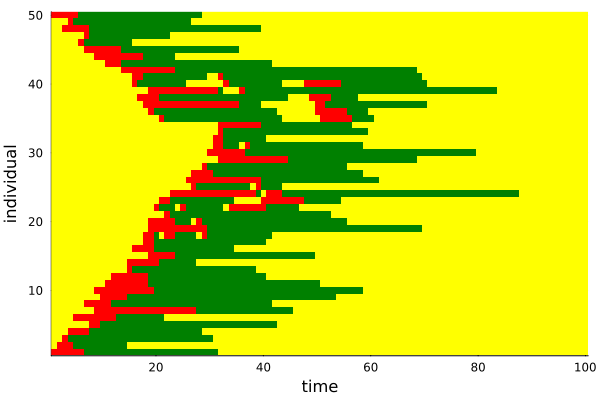
\includegraphics[scale=0.5]{large_example2.png} }	
\only<3>{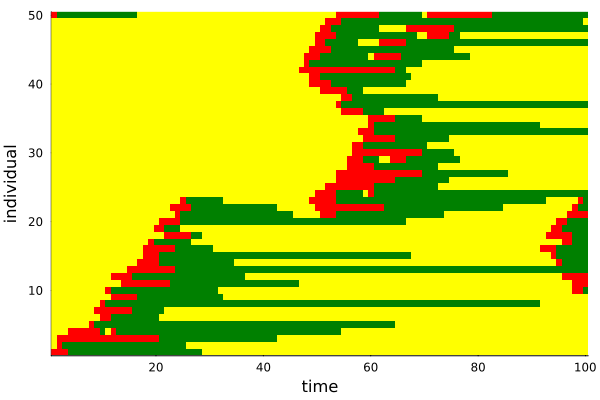
\includegraphics[scale=0.5]{large_example3.png} }	
\only<4>{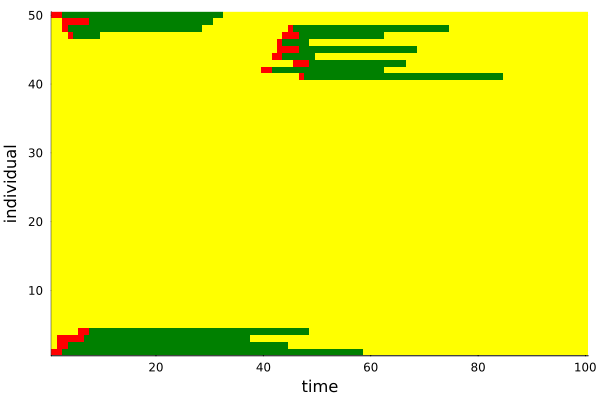
\includegraphics[scale=0.5]{large_example4.png} }	
\only<5>{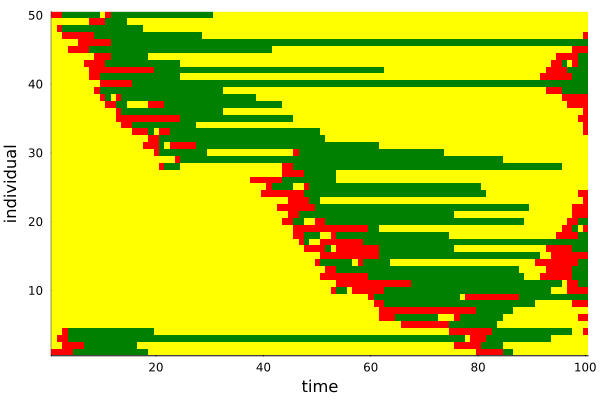
\includegraphics[scale=0.5]{large_example5.png} }	
\only<6>{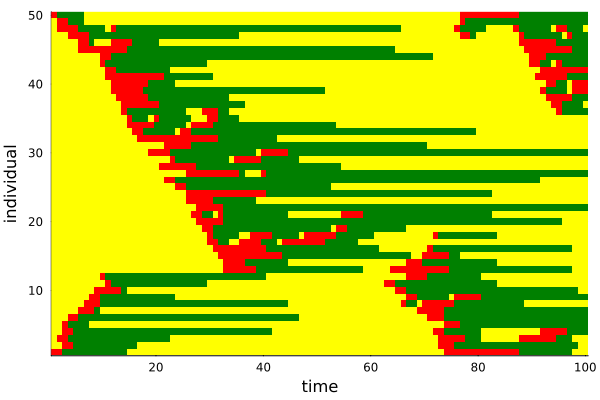
\includegraphics[scale=0.5]{large_example6.png} }	
\only<7>{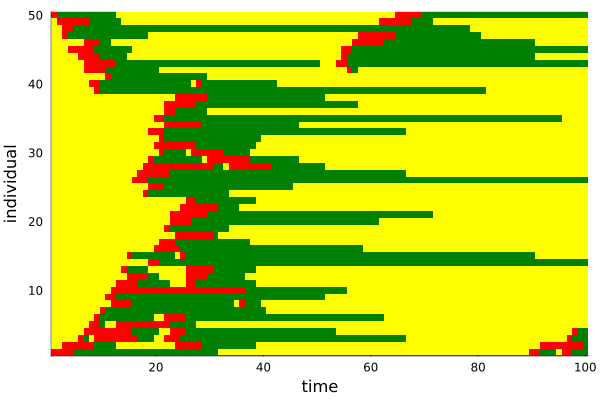
\includegraphics[scale=0.5]{large_example7.png} }	
\only<8>{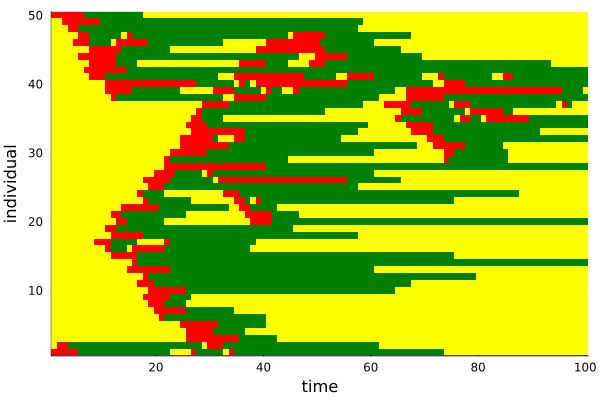
\includegraphics[scale=0.5]{large_example8.png} }	
\end{frame}

\begin{frame}{Als we sneller gemiddeld 3x zo snel weer susceptible zijn na recovered}

\only<1>{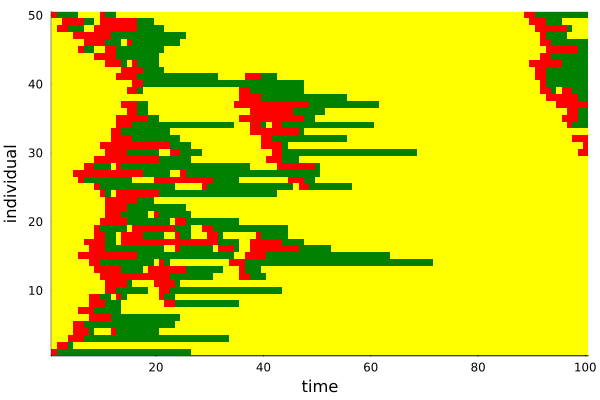
\includegraphics[scale=0.5]{large_example_faster_susceptible1.png} }
\only<2>{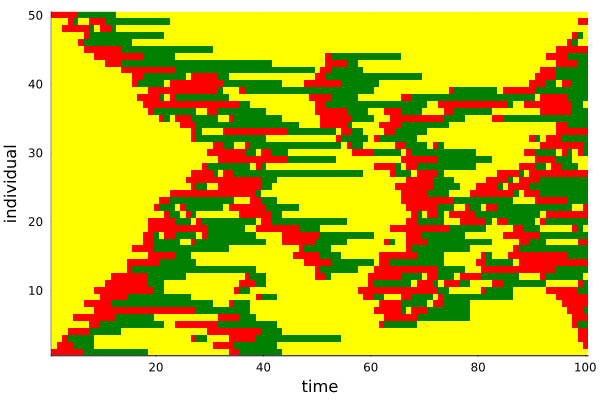
\includegraphics[scale=0.5]{large_example_faster_susceptible2.png} }	
\only<3>{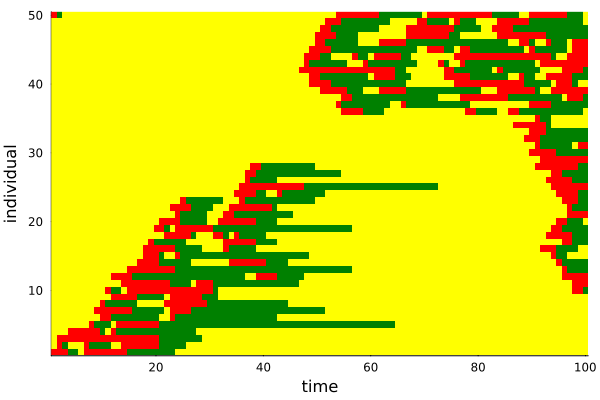
\includegraphics[scale=0.5]{large_example_faster_susceptible3.png} }	
\only<4>{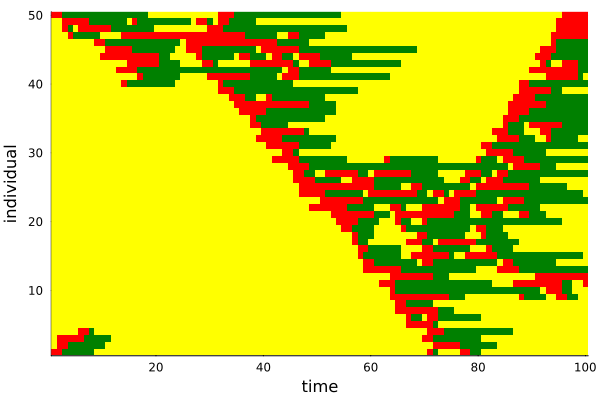
\includegraphics[scale=0.5]{large_example_faster_susceptible4.png} }	
\only<5>{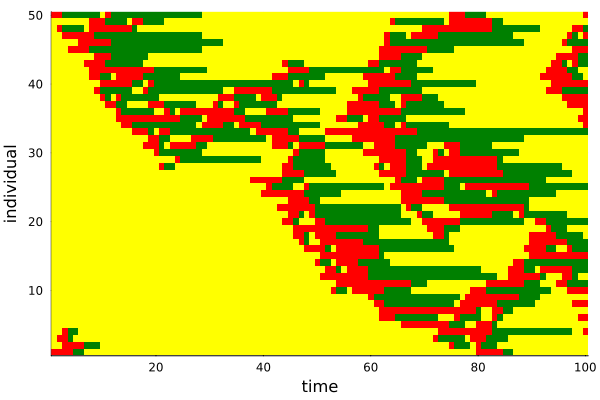
\includegraphics[scale=0.5]{large_example_faster_susceptible5.png} }	
\only<6>{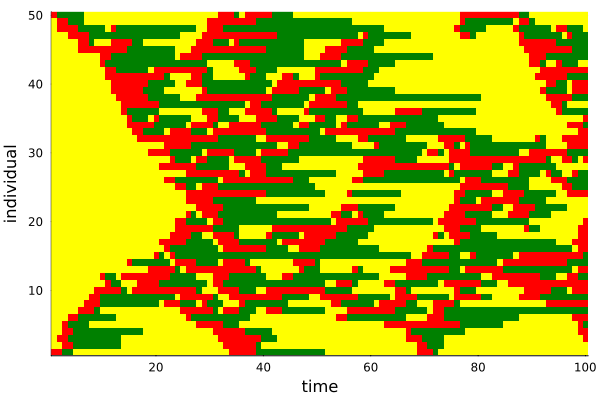
\includegraphics[scale=0.5]{large_example_faster_susceptible6.png} }	
\only<7>{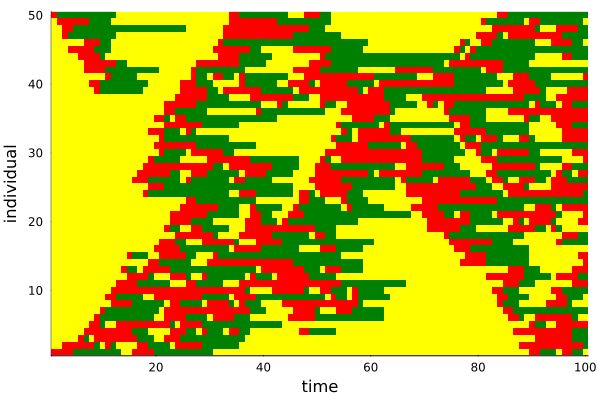
\includegraphics[scale=0.5]{large_example_faster_susceptible7.png} }	
\only<8>{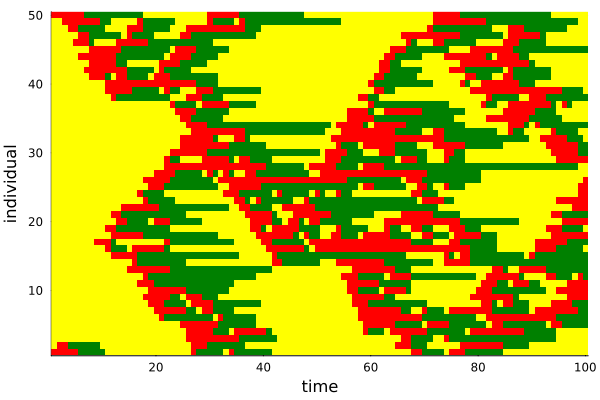
\includegraphics[scale=0.5]{large_example_faster_susceptible8.png} }	

	
\end{frame}


\begin{frame}{We krijgen niet alle informatie}

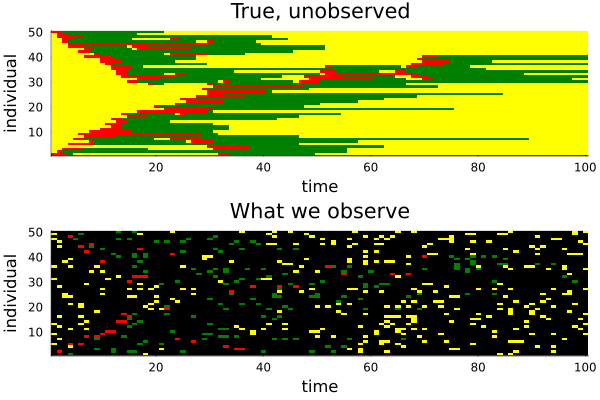
\includegraphics[scale=0.5]{large_example_forw_and_observe.png}
	
\end{frame}
	
	
\begin{frame}{Het invullen van de kleurplaat heeft vele mogelijkheden}

\begin{itemize}
	\item $50 \times 100=5000$ vakjes.
	\item $3^{5000}$ mogelijkheden?
\end{itemize}

	
\end{frame}
	
	
\end{document}
